\chapter{Electron beam size measurements with
direct spikes measurements of synchrotron radiation at free-electron laser facilities}
\label{chapter:CUCTUS}

    In this chapter, I present the results of measuring the electron beam size at the European XFEL free-electron laser facility using the intensity non-interferometry technique with synchrotron radiation. For this technique, it is sufficient to use a synchrotron radiation imager paired with an undulator commissioning crystal monochromator at Bragg's angle. By measuring the transverse intensity correlation, I retrieved the electron beam size at the undulator cell where this radiation was emitted. I tested this technique at the hard X-ray SASE1 and SASE2 beamlines of the European XFEL.

\section{Introduction}

    The method is based on a Hanbury Brown and Twiss-type experimental setup~\cite{cite}, where the subtended size of the radiation is determined by auto-correlating its intensity in the far zone using the results of the van Cittert–Zernike theorem. Following this pioneering experiment by Hanbury Brown and Twiss, this technique spread to various areas of physics research such as~\cite{cite it from Singer's work}. \textit{(To be continued...)}
    
    The Hanbury Brown and Twiss-type experiment not only measured the angular size of Sirius but also implicitly proved that solar radiation is stochastic. Although it has not been conclusively shown until modern times that thermal electromagnetic fields are fluctuating fields~\cite{cite}, both in the time and spatial domains (or their reciprocal pairs), the authors of~\cite{cite} directly demonstrated transverse solar radiation "speckles." Another example of stochastic radiation is SASE FEL radiation. In the FEL community, field fluctuations are referred to as spikes, despite the term speckles being commonly accepted. The motivation for this terminology is that speckles refer to the random interference of coherent light on a statistical object upon propagation, whereas spikes refer to the inherent structure of the radiation source. It was first shown theoretically~\cite{cite} and then experimentally that SASE spectra (a single shot event) consist of spikes, which clearly indicate the randomness of the process. This property is inherited from the shot noise in the electron beam. As SASE essentially starts from synchrotron radiation, one would expect to observe spikes in synchrotron radiation structure too, both in the time and spatial domains. The typical size of the spikes is the corresponding coherence length. So, the goal of this study is to reveal transverse spikes of SR directly and prove that SR is also a fluctuating field in the transverse domain. I depict SASE radiation at the early stages of amplification in Fig.…
    
    \textit{(Insert figure of 3D SASE at start)}
    
    Although it is possible to measure the transverse correlation function of the radiation with interferometric techniques, e.g., double slit, there have not been direct measurements of the single-shot events of the SR radiation that would reveal its fluctuating field. In a remarkable experiment that is presented in~\cite{cite} the authors built a high-resolution monochromator with unprecedented resolving power to resolve SR longitudinal spikes (modes) at the \textit{Spring-8} facility and measure pulse duration. At the time, there was no appropriate imager to detect the transverse distribution of the single-shot events. This experiment was later complemented with measurements of the transverse coherence length~\cite{cite} of synchrotron radiation using a setup similar to the Hanbury Brown and Twiss-type experiment. In this way, the authors retrieved the electron beam size.
    
    In this paper, I present the first measurements of the SR transversely spiky structure. 
    At the moment the present imager at European XFEL did not allows visually determine the spiky content of the recorded events, so I performed the cross-correlation analysis to recover the typical size of the spikes at the images. Then by determining the typical size of these spikes, in other words, the transverse coherence length, I retrieve the electron beam size, similar to what was done in~\cite{rr}. 
    
    I also discuss the practical use of the method for optimizing the FODO lattice and subsequently SASE performance. The recent advancements in creating femtosecond-order pulses~\cite{cite}, or even shorter, at FELs necessitate electron beam diagnostic tools to accurately manipulate the electron beam phase space. This becomes especially important when dealing with transversely tilted electron beams exhibiting a substantial energy chirp. \textit{(Write about HXRSS optimization)}. Under such circumstances, a comprehensive understanding of the transverse electron beam characteristics along the entire FEL undulator line becomes essential for optimizing SASE performance.
    
    This chapter is organized as follows: first, I will estimate the parameter space in terms of the expected contrast of the images I record, as well as the possibility of spatially resolving the sought correlation function. Then, I present the method I utilized to perform correlation analysis. Subsequently, I show the simulation results that replicated the expected radiation behavior. In the real experiment, the signal is so low that the signal-to-noise ratio in most cases falls below unity. Therefore, I upgraded the correlation analysis. This upgrade relies on the fact that the radiation is quasi-homogeneous, allowing for averaging over auto-correlation function anti-diagonals to effectively increase statistics. Finally, I present the experimental results, where I observed a significant level of correlation. I estimated its width and retrieved the electron beam size. I conclude the chapter with a discussion on the possible implementation of the method in BKR of the European XFEL and issues to be addressed in the future.
    
\section{Underlining theory}

\subsection{Qualitative estimations}
    As was mentioned in the introduction synchrotorn radiation possesses spike structure in both domain longitudinal and transverse. As one would detect this radiation  monochromotised and in the far zone it make sense to setup ones thinking in frequency-inverse space domains. In this representation of the radiation each longitudinal spike in the frequency domain will contain its unique transverse spiky distribution in inverse space domain. In essence, the typical width of these spikes is the spectral correlation function, which in other words means that transverse spikes are statistically independent of each other. So, I what one would observe a a convectional synchrotron radiation source based on a storage ring is a smoothed transverse radiation distribution upon monochromatisation. This happens do to relately long of order of dozens pico second electron beam duration that defines that radiation pulse duration as well. As longitudinal coherence length is much less than this pulse duration one would expect to observe immense number of the spikes in longitudinal domain even upon monochromatization with a conventional monochromator. This is the reason why the authors of~\cite{} built such a unique monochromator to resolve spikes in frequency domain, which was essential for their measurements.

    \begin{figure*}[h!]
    	\centering
        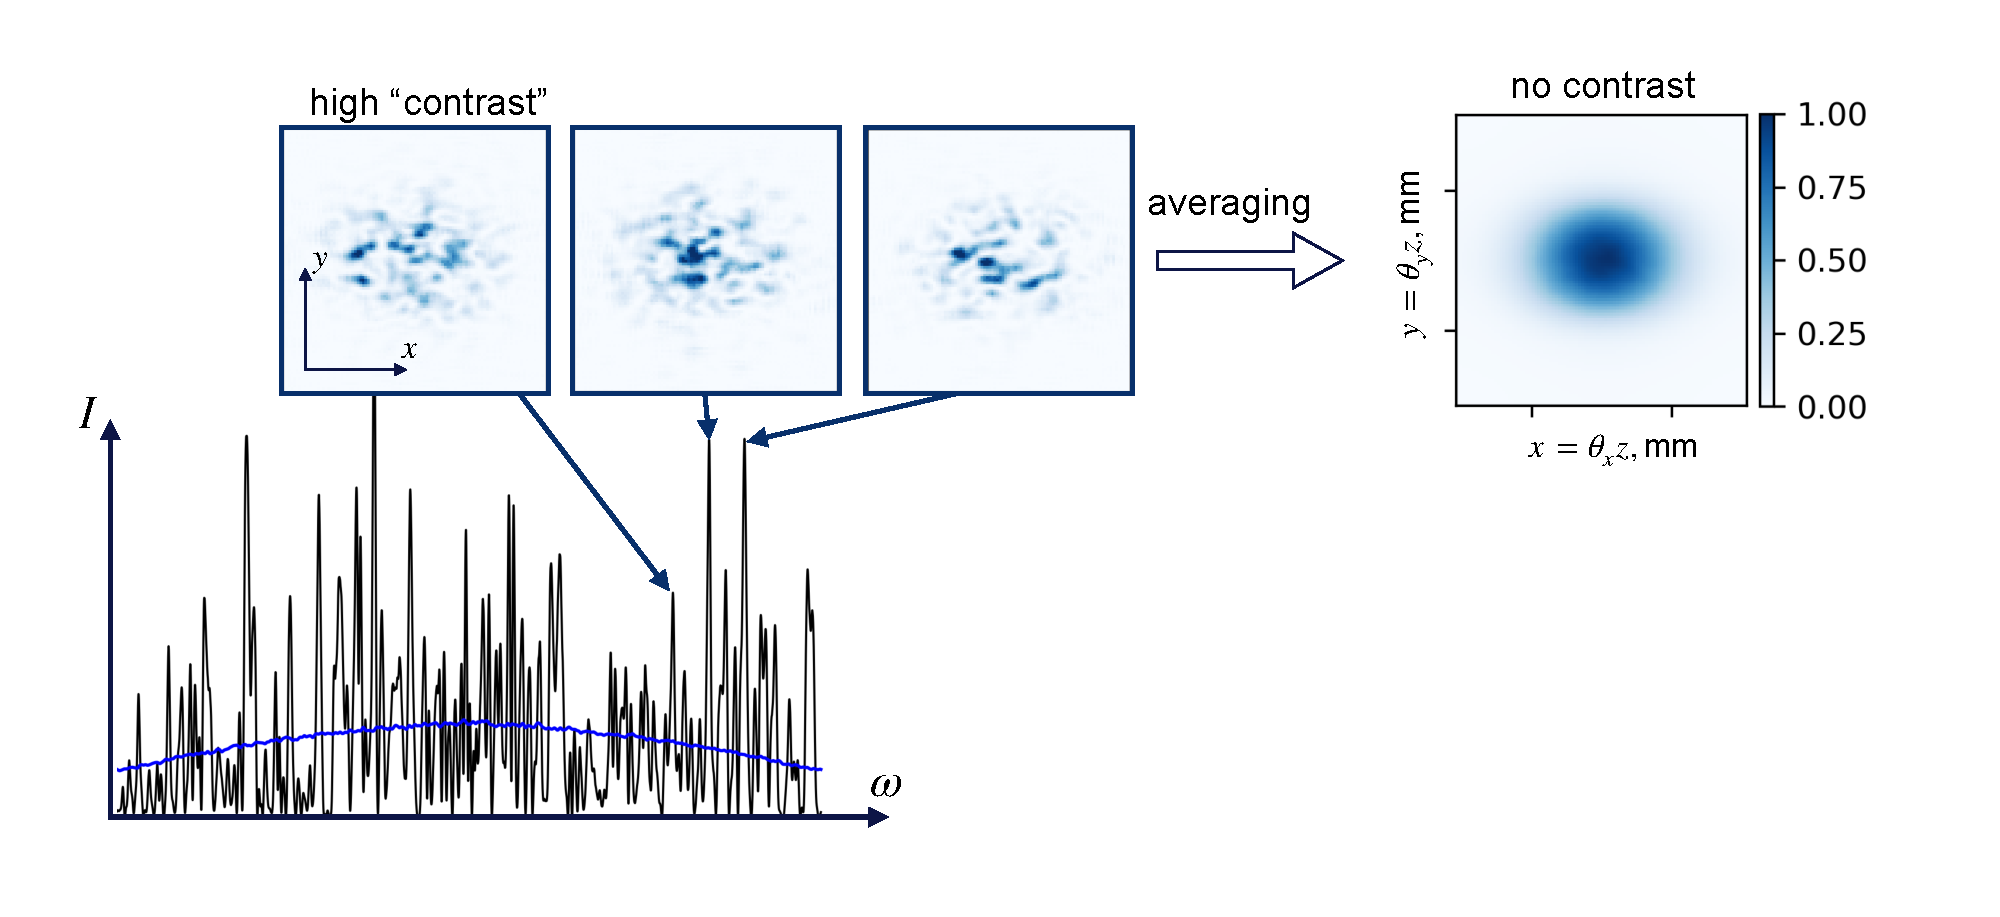
\includegraphics[width=0.99\linewidth]{content/images/ebeam_size_with_SR/SR_spikes_many.pdf}
        \captionsetup{justification=centering}
        \caption{}
        \label{Fig:SR_spikes_many}
    \end{figure*}

    The situation is radically different parametrically-wise at linear accelerator facilities such as European XFEL. The duration of the electron beam are at the dozen of femtosecond level. This why if one use just a single undulator cell to generate usual synchrotron radiation there will be much fewer longitudinal spike upon monochromatisation with a conventional crystal monochromator with Si~(111) reflection, as shown in Fig.~\ref{Fig:SR_spikes_few}. Then at an imager one would observe effective averaging of the spikes distribution that are contained in the longitudinal spikes. As a result averaging over several dozens of the longitudinal spikes will result in a low contrast transverse distribution, that will still will contain the imprint of the spikes, what I show in Fig.~\ref{Fig:SR_spikes_few} in the red-framed subplot. This result is only possible with an ideal imager, in real case scenario the resulting image may be heavily affected by noise.

    \begin{figure*}[h!]
    	\centering
        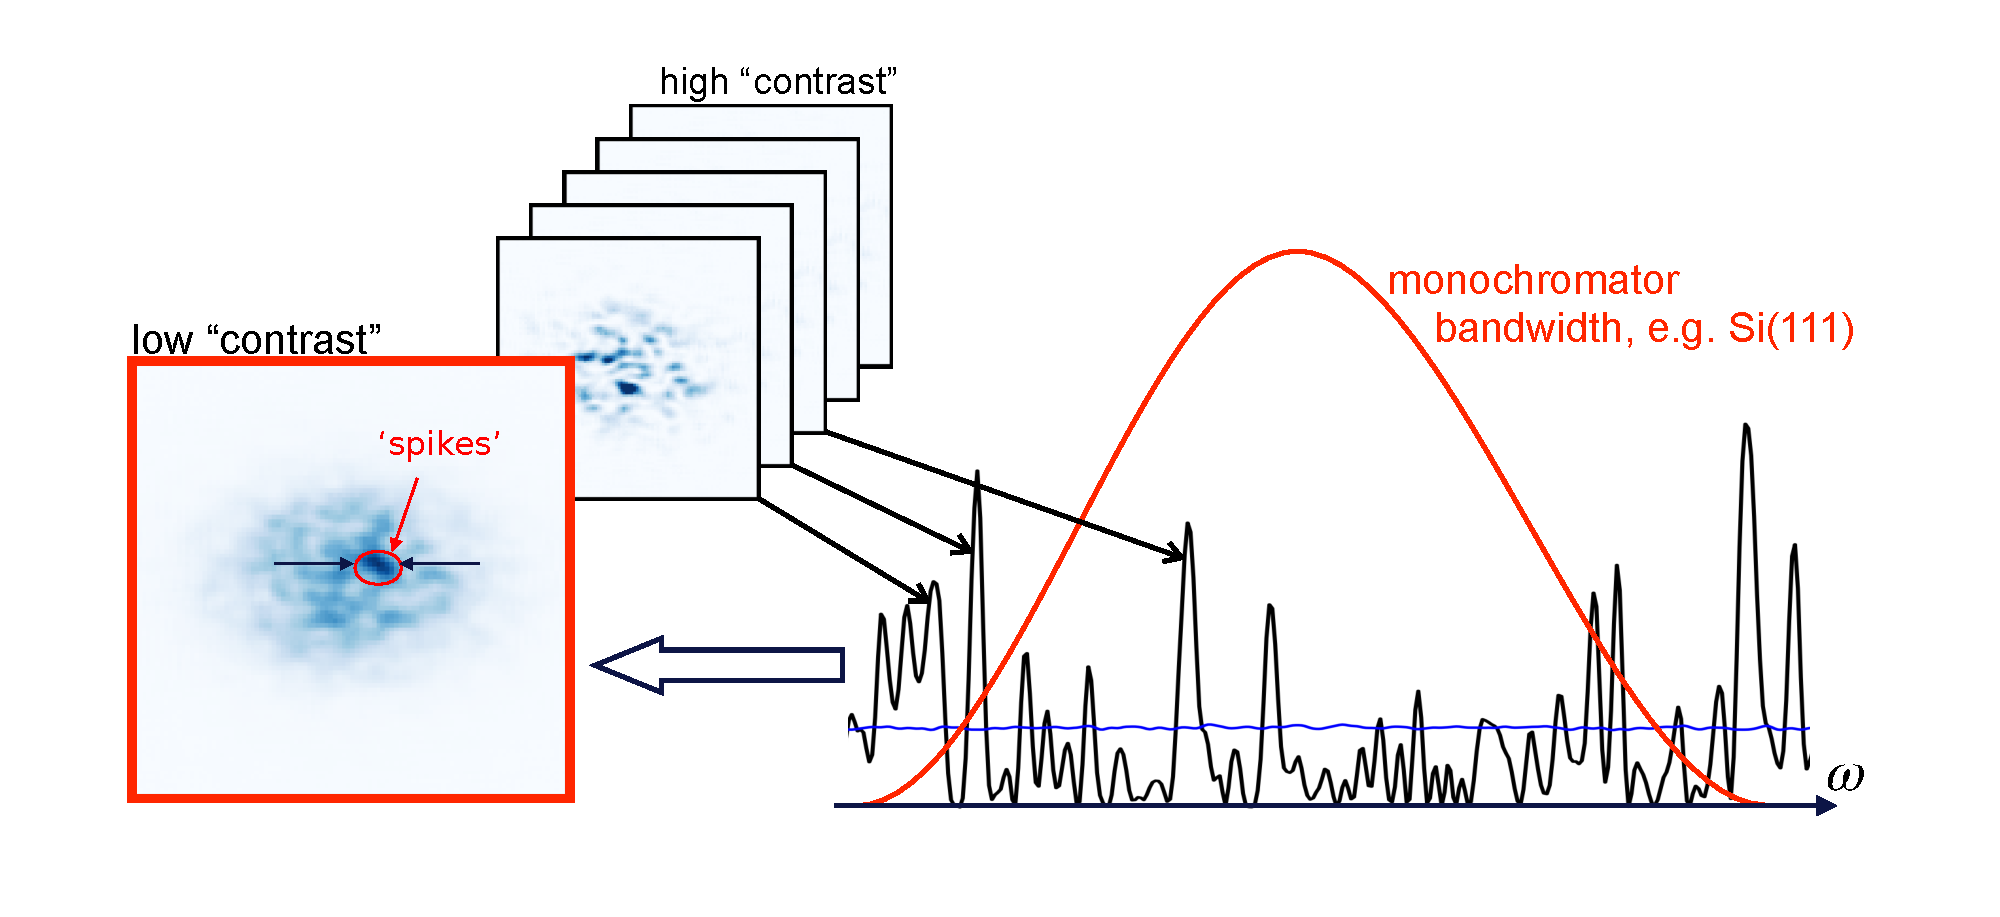
\includegraphics[width=0.99\linewidth]{content/images/ebeam_size_with_SR/SR_spikes_few.pdf}
        \captionsetup{justification=centering}
        \caption{}
        \label{Fig:SR_spikes_few}
    \end{figure*}

    So, is one collect enough statistic of these averaged images and then calculate the typical size of these spikes then on would be able tho retrieve the electron beam size. Before proceeding to this analysis part I will provide more qualitative estimation on the expected contrast of the image and required spatial resolution of the imager.
    
\subsection{Quantitative estimations}
    At first I estimate number of longitudinal spike that on cut out with a silicon based monochromator under Brag's angle using (111) reflection. Knowing typical spike width and the resolution of Si~(111) I plot the dependence of the amount of spike extracted with the monochromator versus pulse duration and undulator radiation resonance frequency in Fig.~\ref{Fig:M_L} calculated with Eq.~\ref{Eq:M_L}:
    \begin{align}
        M_L = \cfrac{2\sqrt{2 \textup{ln}(2)} \sigma_{ebeam} \Delta E}{h}.
        \label{Eq:M_L}
    \end{align}
    
    \begin{figure*}[h]
    	\centering
        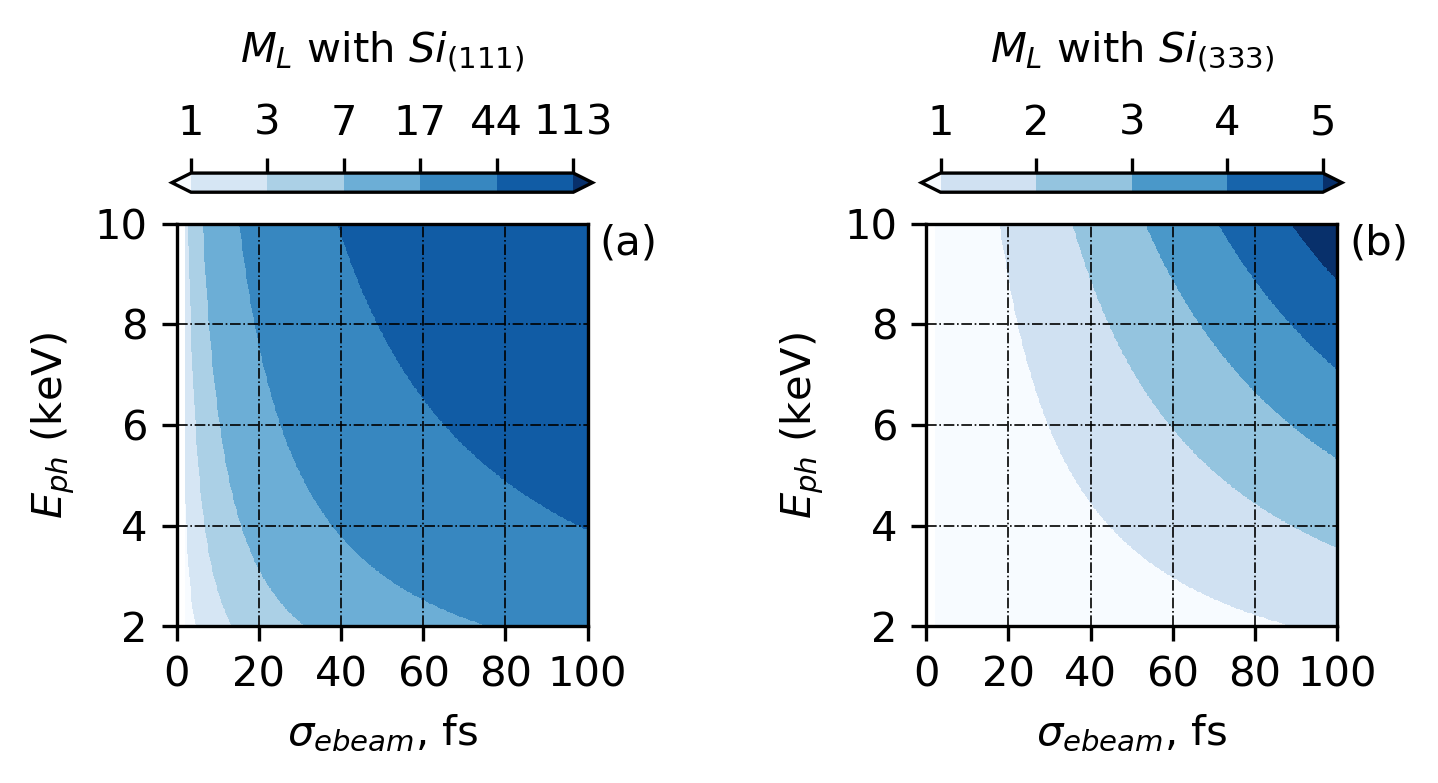
\includegraphics[width=0.63\linewidth]{content/images/ebeam_size_with_SR/M_L.png}
        \captionsetup{justification=centering}
        \caption{}
        \label{Fig:M_L}
    \end{figure*}

    In term of the spacial resolution required to resolve the correlation function I plot the distributions in Figs.~\ref{Fig:cell_2},~\ref{Fig:cell_18}, and~\ref{Fig:cell_37} where I depict the resulting correlation function versus electron beam transverse size and used undulator radiation  resonance frequency.
    \begin{figure*}[h!]
        \centering
        \begin{subfigure}[b]{0.32\textwidth}
            \centering
            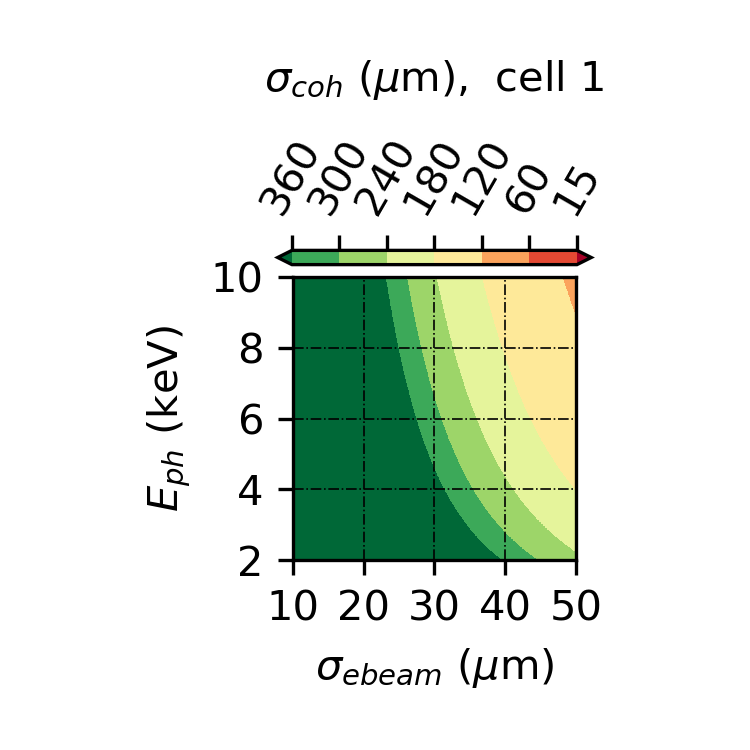
\includegraphics[trim={0.4cm 0 0.4cm 0}, clip, width=\textwidth]{content/images/ebeam_size_with_SR/cell 1.png}
            \caption{Caption for the first figure}
            \label{Fig:cell_2}
        \end{subfigure}
        \hfill % Use \hfill to add horizontal space between figures
        \begin{subfigure}[b]{0.32\textwidth}
            \centering
            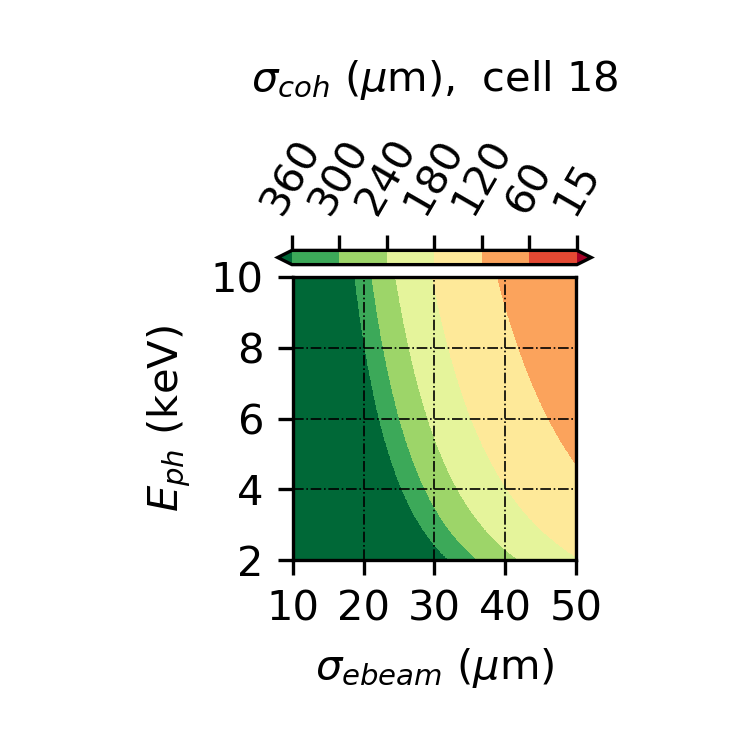
\includegraphics[trim={0.4cm 0 0.4cm 0}, clip, width=\textwidth]{content/images/ebeam_size_with_SR/cell 18.png}
            \caption{Caption for the second figure}
            \label{Fig:cell_18}
        \end{subfigure}
        \hfill % Use \hfill to add horizontal space between figures
        \begin{subfigure}[b]{0.32\textwidth}
            \centering
            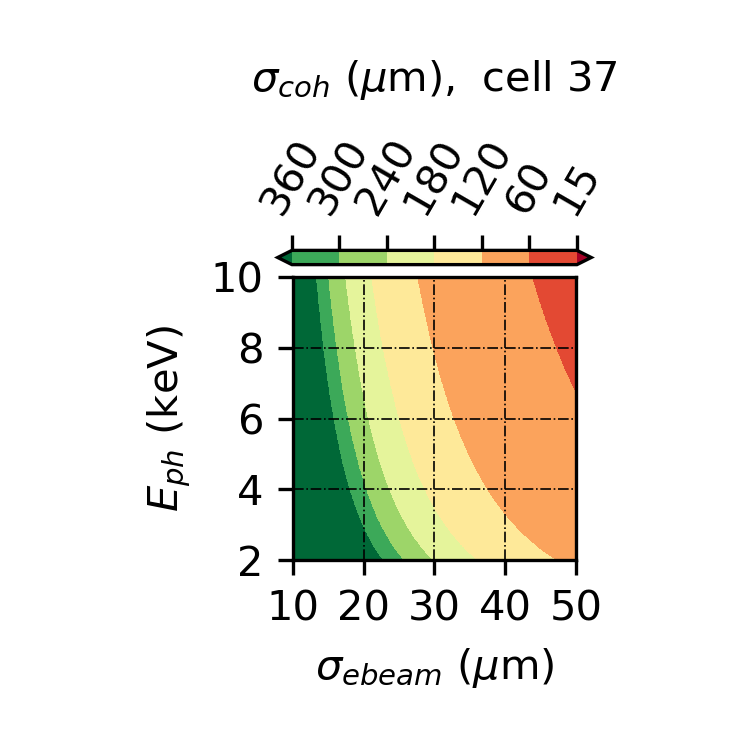
\includegraphics[trim={0.4cm 0 0.4cm 0}, clip, width=\textwidth]{content/images/ebeam_size_with_SR/cell 37.png}
            \caption{Caption for the third figure}
            \label{Fig:cell_37}
        \end{subfigure}
        \caption{General caption for all figures.} % Optional: General caption for all subfigures
    \end{figure*}
    It is clear from these estimations that it is more then possible to see spikes in transverse dimension after monochromatization. In the next section I will show the simulation of the real experiment that was conducted at European XFEL. I also in detail describe the raw data processing procedures to extract information about the correlation function.
    
\section{Simulation}
    I replicated the experimental results in the simulation using SERVAL algorithm presented before in the thesis. In Fig.~\ref{Fig:int_corr_1event} I present 
    \begin{figure}[h!]
    	\centering
        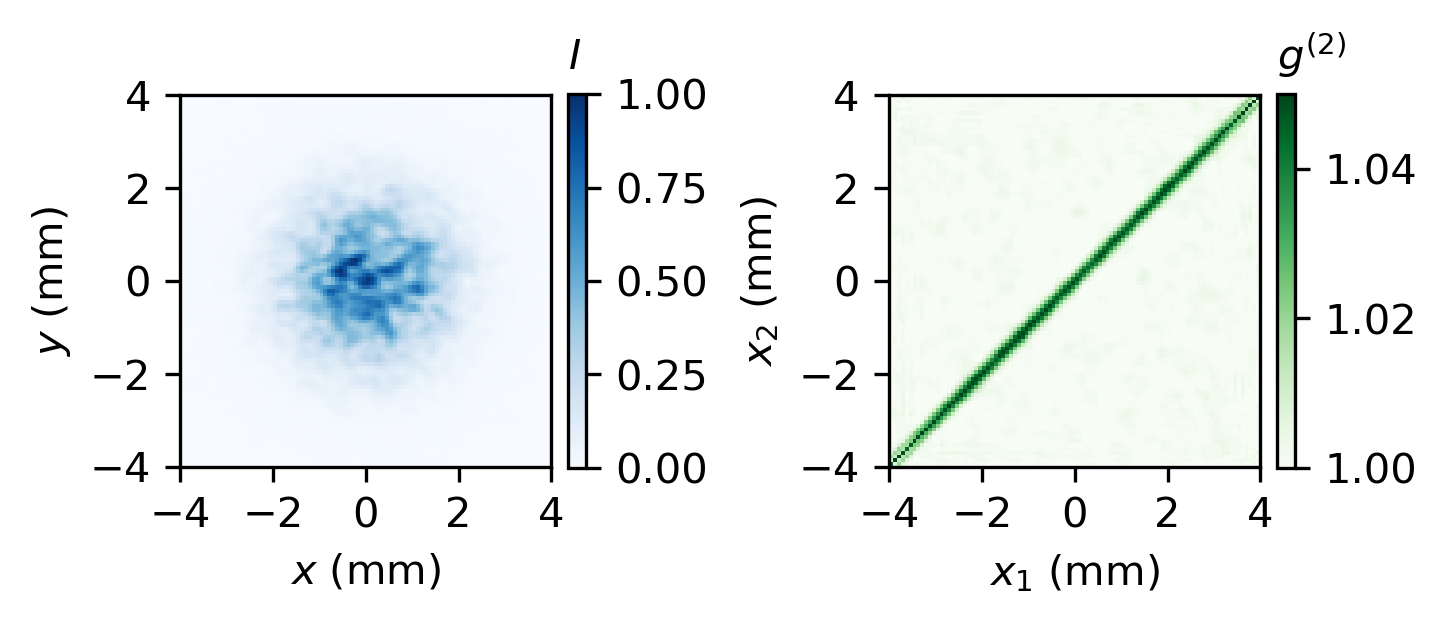
\includegraphics[width=0.66\linewidth]{content/images/ebeam_size_with_SR/int_corr_1event.png}
        \captionsetup{justification=centering}
        \caption{}
        \label{Fig:int_corr_1event}
    \end{figure}

    \begin{figure}[h!]
    	\centering
        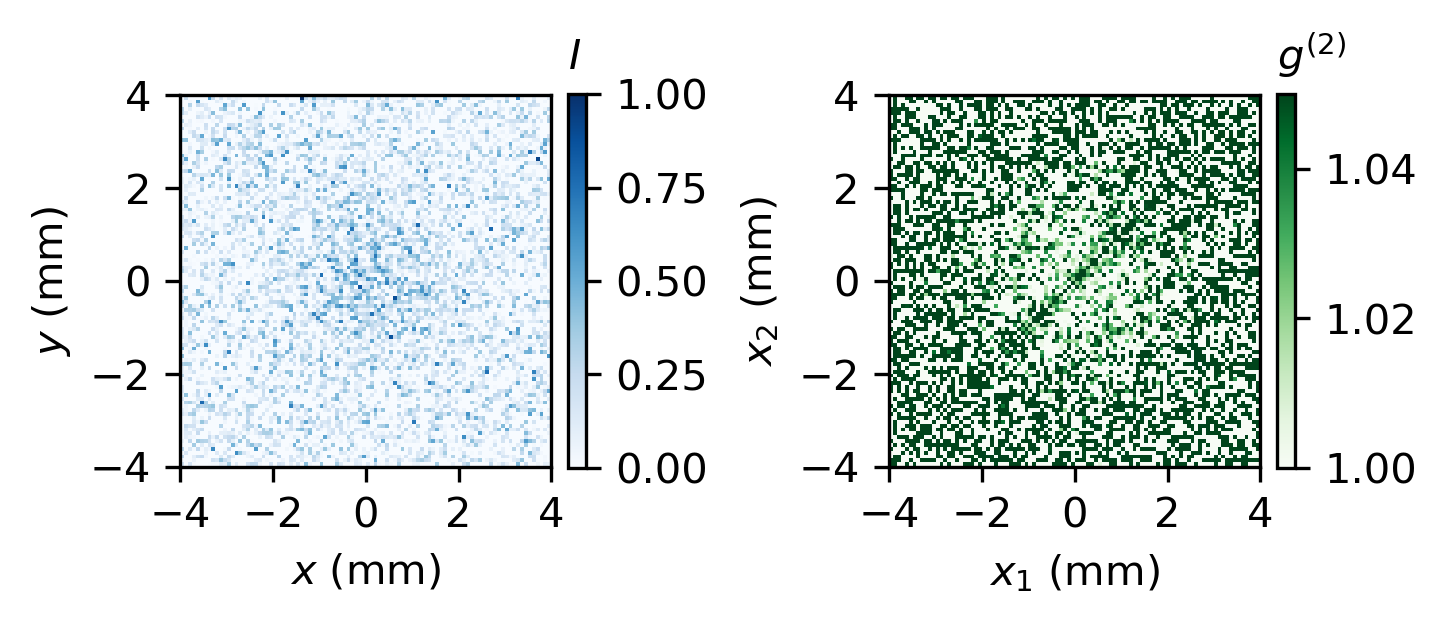
\includegraphics[width=0.66\linewidth]{content/images/ebeam_size_with_SR/int_corr_1event_noise.png}
        \captionsetup{justification=centering}
        \caption{}
        \label{Fig:int_corr_1event_noise}
    \end{figure}

    \begin{figure}[h!]
    	\centering
        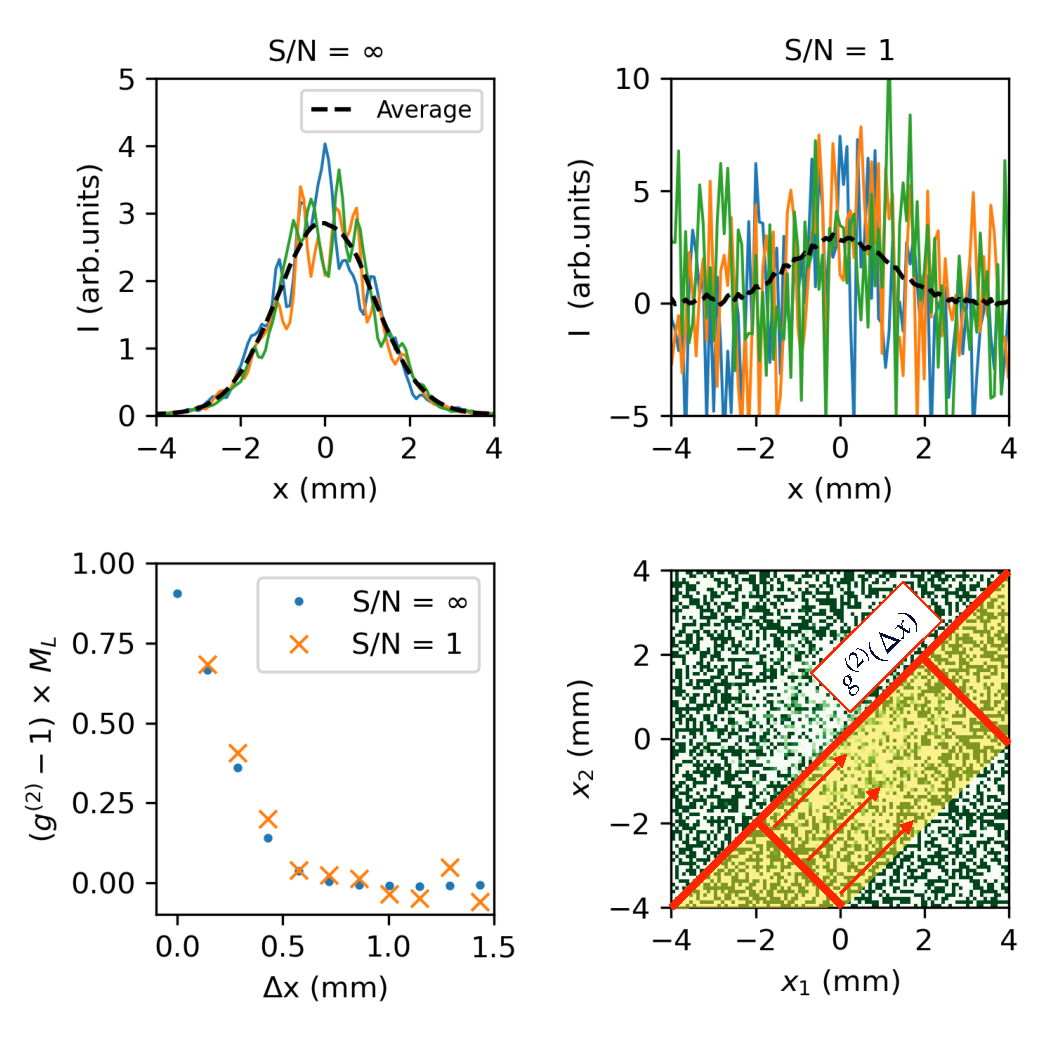
\includegraphics[width=0.66 \linewidth]{content/images/ebeam_size_with_SR/triangle_mod_full.pdf}
        \captionsetup{justification=centering}
        \caption{}
        \label{Fig:triangle}
    \end{figure}
\section{Experimental results}

    The experiment for measured the transverse coherence of SR at European XFEL was done at SASE1 and SASE2 beamlines of the facility. This beamlimes are equipped with K-mono -- a undulator commissioning monochromator --, and a SR imager. 
    
    
\section{Outlook and discussion}

\section{Conclusion}